% view link
% https://www.overleaf.com/read/kvwrsvwmmgnb
\RequirePackage{xcolor}
\documentclass{ipol}

\ipolSetTitle{IPOL Template}
\ipolSetAuthors{Authors}

\ipolSetAffiliations{Universit\'e Paris-Saclay, ENS Paris-Saclay, Centre Borelli, F-91190 Gif-sur-Yvette, France \\
\texttt{\{first.last\}@ens-paris-saclay.fr}} % change as needed

% Below: replace XXXXXXXX with your demo ID
\ipolPreprintLink{https://ipolcore.ipol.im/demo/clientApp/demo.html?id=XXXXXXXX}

% Below: only for accepted publications
%\ipolSetID{355}
%\ipolSetVolume{11}

%\ipolSetSubmissionYear{2021}
%\ipolSetSubmissionMonth{05}
%\ipolSetSubmissionDay{05}

%\ipolSetAcceptedYear{2021}
%\ipolSetAcceptedMonth{08}
%\ipolSetAcceptedDay{24}

%\ipolSetPublicationYear{2021}
%\ipolSetPublicationMonth{10}
%\ipolSetPublicationDay{15}


%\setcounter{page}{317}


%new format (2017) for figures and table captions
\usepackage[font={sf,footnotesize}]{caption}

\usepackage{hyperref,graphicx,amsmath,amssymb,amsthm}
\usepackage{url}

\usepackage{subcaption}
\usepackage{soul}
\usepackage{colortbl}
\usepackage{booktabs}
\usepackage[vlined,algoruled,linesnumbered]{algorithm2e}
\usepackage{multirow}


% Below: pseudocode definitions
% Pseudocode is needed for standard IPOL articles,
% but not for Brief articles. If you are doing a 
% Brief article, you can remove it
% This is only one of the naming conventions, there are
% no set standards. Feel free to edit those for your demo
% namedinput: custom package to allow inputs and outputs in the shape "Input foo: description", rather than the default "Input: description". Again, feel free to edit namedinput.sty or remove the package entirely
\usepackage{namedinput}
\definecolor{commentcolor}{HTML}{0E918C} % again, just a suggestion
\SetKwNamedIO{Input}{Input}
\SetKwNamedIO{Parameter}{Param}
\SetKwNamedIO{Output}{Output}
\SetKwProg{Function}{function}{}{}
\SetKwComment{Comment}{\color{commentcolor}\# }{}
\renewcommand{\CommentSty}[1]{\textnormal{\ttfamily\color{commentcolor}#1}\unskip}
\newcommand{\assign}{:\!=}
\newcommand{\peq}{+\mkern-8mu=} % to write += correctly
\newcommand{\meq}{-\mkern-8mu=}
\DontPrintSemicolon
% Useful keywords, to call with, e.g. \IN. Again, use your own if you want.
% \SetKw{command}{keyword} will allow you to output "keyword" in algorithms with \command. Avoid using common names for \command that might clash with other LaTeX commands. Using all-caps seems to help avoid that
\SetKw{IN}{in}
\SetKw{AND}{and}
\SetKw{FROM}{from}
\SetKw{TO}{to}


\begin{document}


\begin{ipolAbstract}
Write your abstract here.
\end{ipolAbstract}

% do not modify this
\begin{ipolCode}
The reviewed source code and documentation for this algorithm are
available from \href{\ipolLink}{the web page of this
article}. Usage instruction are included in the
\verb|README.txt| file of the archive.
\end{ipolCode}



\ipolKeywords{keywords; semi-colon; separated}


\section{Example algorithm}

\begin{algorithm}[!htb]
\caption{\label{alg:example} Example algorithm}
\Function{my\_function(foo)}{
\Input{foo}{The input to the function}
\Output{bar}{The output to the function}
$x \assign \texttt{other\_function}(foo)$\;
\For{$i$ \FROM 1 \TO $x$}{
    \For{$m$ \FROM 1 \TO $X$ \AND $n$ \FROM 1 \TO $Y$}{
        $y \assign m+n$\;
        \If{$x\ge y$}{
        $x \peq 2$\;
        }
        \Else{
        $x \meq 1$\;
        }
    }
}
\Return{$x$}
}
\end{algorithm}

\section*{Acknowledgment}
Add acknowledgments here


\section*{Image Credits}
{
\small\flushleft


\small\flushleft
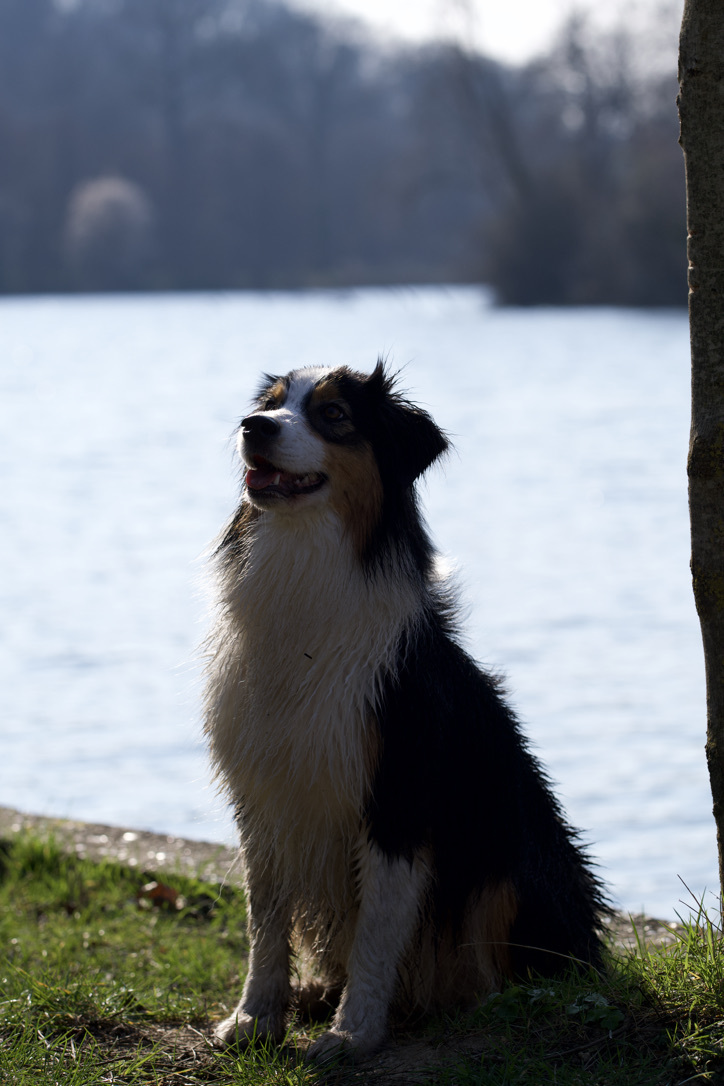
\includegraphics[height=2em]{images/tina0.jpeg}
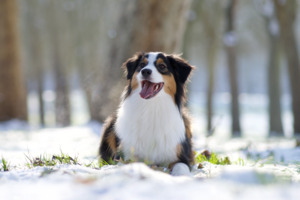
\includegraphics[height=2em]{images/tina1.jpeg} Tina Nikoukhah, with permission from the photographer, processed with libraw~\footnote{LibRaw library, Copyright  \copyright 008-2019 LibRaw LLC, \url{https://www.libraw.org}}
}

\small\flushleft

\includegraphics[height=2em]{images/image0.jpeg}

\includegraphics[height=2em]{images/image1.png} Dataset X (cite)

%------------------------------------------------------------------------------
\bibliographystyle{siam}
\bibliography{biblio}

\end{document}






